\documentclass[14pt]{extarticle}
\usepackage[utf8]{inputenc}
\usepackage[T1, T2A]{fontenc}
% \usepackage{fontspec}
% \setmainfont{Times New Roman}
\usepackage[english, russian]{babel}
\usepackage[a4paper,left=3cm,right=1.5cm,top=2cm,bottom=2cm]{geometry}
\usepackage{graphicx}
\usepackage{subcaption}
\usepackage{changepage}
\usepackage{indentfirst}
\usepackage[intlimits]{amsmath}
\usepackage{amssymb}
\usepackage[titles]{tocloft}
\usepackage{titlesec}
\usepackage{rmathbr}
\usepackage{float}
\usepackage{relsize}
\usepackage{setspace}
\usepackage{anyfontsize}
\usepackage{minted}
\usepackage{enumitem}

\setcounter{secnumdepth}{0}
\setlist{nosep}
\titleformat{\section}{\large\bfseries\filcenter}{}{1em}{}


\newcommand{\Rb}{\mathbb{R}}
\newcommand*{\hm}[1]{#1\nobreak\discretionary{}{\hbox{$\mathsurround=0pt #1$}}{}}
\newcommand{\sectionbreak}{\clearpage}
\newcommand{\dd}{\,\mathrm{d}}
\newcommand{\pvec}{p_{\boldsymbol{\xi}}}
\addto\captionsrussian{\renewcommand{\refname}{Список использованной литературы}}
\renewcommand{\cftsecleader}{\cftdotfill{\cftdotsep}}
\relpenalty=10000
\binoppenalty=10000

\graphicspath{{./images/}}


\begin{document}

    \begin{titlepage}
    \begin{center}
        \textbf{\textscale{0.9}{БЕЛОРУССКИЙ ГОСУДАРСТВЕННЫЙ УНИВЕРСИТЕТ\\[0.2cm]
        ФАКУЛЬТЕТ ПРИКЛАДНОЙ МАТЕМАТИКИ И ИНФОРМАТИКИ\\[0.2cm] }
        Кафедра математического моделирования и анализа данных
        }

        \vspace{4cm}
        \textbf{Отчет\\[0.4cm]
        о прохождении производственной (преддипломной) практики
        }
    \end{center}

    \vfill

    \begin{flushleft}
        \begin{adjustwidth}{7.2cm}{}
            Толочко Александра Викторовича\\[0.3cm]
            студента 4 курса,\\
            специальность Прикладная математика»\\[0.4cm]
            Руководитель практики:\\[0.3cm] 
            кандидат физ.-мат. наук,\\
            доцент И.А. Бодягин
        \end{adjustwidth}
    \end{flushleft}

    \vfill

    \begin{center}
        Минск, 2025
    \end{center}
\end{titlepage}

\begin{center}
    БЕЛОРУССКИЙ ГОСУДАРСТВЕННЫЙ УНИВЕРСИТЕТ\\[0.2cm]
    Факультет прикладной математики и информатики\\[0.2cm]
\end{center}
Кафедра $\underset{\text{(наименование кафедры)}}{\underline{\hspace{8cm}}}$

\vspace{1cm}
\hspace*{8cm}\textbf{Утверждаю}\\[0.2cm]
\hspace*{5cm}Заведующий кафедрой $\underset{\text{(подпись)(фамилия, инициалы)}}{\underline{\hspace{6cm}}}$\\[0.6cm]
\hspace*{10.8cm}<<$\underline{\hspace{0.5cm}}$>>$\underline{\hspace{3cm}}$20$\underline{\hspace{0.5cm}}$г.

\vspace{0.4cm}
\begin{center}
    \textbf{Задание на практику}\\[0.3cm]
    \textbf{по специальности <<Прикладная математика>>}
\end{center}
\begin{flushleft}
    {Студенту $\underset{\text{(фамилия, инициалы)}}{\underline{\hspace{6cm}}}$

    \vspace{0.6cm}
    1. Тема практики: $\underset{\text{(наименование темы дипломной работы)}}{\underline{\hspace{10cm}}}$\\

    \vspace{0.6cm}
    2. Список рекомендуемой литературы:\\
    \hspace*{0.8cm}2.1. Андерсон, Т. Статистический анализ временных рядов\\
    \hspace*{0.8cm}2.2. Дженкинс, Г., Ваттс, Д. Спектральный анализ и его приложения: в 2 т.\\
    \hspace*{0.8cm}2.3. Бокс Дж., Дженкинс Г. Анализ временных рядов, прогноз и управление\\
    \hspace*{0.8cm}2.4. Харин, Ю.С. Оптимальность и робастность в статистическом
    прогнозировании\\[0.3cm]

    3. Перечень подлежащих разработке вопросов или краткое содержание расчетно-пояснительной записки:\\[0.2cm]
    \hspace*{0.8cm}3.1. Исследовать применимость метода игнорирования пропусков в случае
    пропусков, зависящих от данных\\[0.2cm]
    \hspace*{0.8cm}3.2. Показать, как модель неслучайных пропусков влияет на работу стандартных
    методов оценивания параметров\\[0.2cm]
    \hspace*{0.8cm}3.3. Получить верные оценки параметров распределения в случае пропусков, 
    зависящих от данных\\[0.3cm]

    4. Примерный календарный график:\\[0.2cm]
    \begin{itemize}
        \item[$-$] \textbf{февраль (1-ая неделя)} $-$ ознакомление с условиями работы,
        изучение основных теоретических вопросов, получение задания.
        \item[$-$] \textbf{февраль (2-3-я неделя)} $-$ построение модели для описания различных 
        видов пропусков.
        \item[$-$] \textbf{март (4-5-ая неделя)} $-$ исследование метода максимального правдоподобия для получения оценки
        в случае пропусков, зависящих от данных.
        \item[$-$] \textbf{март (6-7-ая неделя)} $-$ исследование метода моментов для получения оценки
        в случае пропусков, зависящих от данных.
        \item[$-$] \textbf{апрель (8-9-ая неделя)} $-$ проведение комрьютерных экспериментов для
        проверки полученных результатов.
        \item[$-$] \textbf{апрель (10-ая неделя)} $-$ обобщение результатов и подготовка отчета
    \end{itemize}

    \vspace{0.4cm}
    5. Руководители практики:\\[0.2cm]
    \hspace*{0.2cm}от предприятия $\underset{\text{(ФИО)}}{\underline{\hspace{8cm}}}$\\[0.1cm]
    \hspace*{0.2cm}от кафедры $\underset{\text{(ФИО)}}{\underline{\hspace{8cm}}}$\\[0.3cm]

    \vspace{0.6cm}
    6. Дата выдачи задания \hspace{0.2cm} $\underline{\hspace{4cm}}$\\[0.2cm]

    7. Срок сдачи отчета \hspace{0.88cm} $\underline{\hspace{4cm}}$\\[0.6cm]
    
    {\small $\underset{\text{(от кафедры)}}{\text{Руководитель}} \underset{\text{(подпись)}}{\underline{\hspace{3cm}}}\;\underset{\text{(инициалы, фамилия)}}{\underline{\hspace{6cm}}}$\\[0.6cm]
    Подпись студента $\underset{\text{(подпись, дата)}}{\underline{\hspace{6cm}}}$}
    
    }
\end{flushleft}

    \tableofcontents

    \section{Введение}

    Временной ряд представляет собой набор наблюдений, полученных путем регулярного измерения одной переменной
    в течение некоторого периода времени. Наблюдения представляют собой набор из одного или нескольких значений, 
    зафиксированных в определенный момент времени. Элементами наблюдения являются действительные числа --- значения 
    непрерывных или дискретных переменных.

	Временные ряды --- один из наиболее важных инструментов в аналитике данных. Они используются во многих областях, 
    включая финансы, производство, социальные и экономические исследования, климатологию и другие. Примеры временных 
    рядов могут включать данные о продажах продукции в определенный день или данные о температуре на определенной 
    территории в различные временные промежутки.

	На практике зачастую часть значений переменных во временном ряду по какой-то причине отсутствует. Например, 
    часть респондентов, участвующих в обследовании семей, может отказаться сообщить размер дохода. Пропуски также 
    могут быть вызваны факторами, не связанными с самим экспериментальным процессом, например, ограничения или 
    неисправности оборудования, собирающего данные.
    
    Существуют множество видов пропусков, но в литературе наиболее часто встречаются следующие:
    \begin{itemize}
        \item Случайные пропуски --- пропуски, не зависящие от данных и от самого эксперимента (второй пример 
        из приведенных выше)
        \item Цензурирование --- пропуски, зависящие от данных, при которых пропускаются лишь значения из определенной 
        области. Цензурирование называется полным, если пропускаются все значения из области (в качестве примера 
        можно взять исследование сроков наступления эффекта лекарства, в котором все значения, большие срока 
        проведения эксперимента, будут пропущены). Цензурирование называется частичным если лишь часть значений из 
        области пропускается (пример с размером дохода в опросе семей).
    \end{itemize}

    При работе с пропусками, зависящими от данных, могут возникнуть серьезные проблемы, так как в этом случае 
    большинство рядовых методов, используемых для статистического анализа временных рядов, как игнорирование 
    пропусков, оказываются неэффективными, что будет подтверждено в ходе курсового проекта. Поэтому необходимо 
    использование иных методов, основывающихся на некоторой определенной модели пропусков или на более общей модели.


    \section{Математическая модель и постановка задачи}

    Пусть наблюдается выборка
    \begin{equation*}
        X = (x_1, x_2, \dots , x_T), \quad x_i \in \Rb ,
    \end{equation*}
    из некоторого абсолютно непрерывного закона распределения вероятности с плотностью $p_\xi$, заданной с точностью 
    до параметров. И пусть некоторые значения выборки пропущены, то есть известно, что на 
    данном месте должно наблюдаться некоторое значение, но само оно неизвестно. В литературе чаще всего встречаются 
    два основных вида пропусков во временных рядах по зависимости от данных:
    \begin{enumerate}
        \item Случайные пропуски (не зависят от данных)
        \item Цензурирование (зависят от данных)
    \end{enumerate}

    Обобщим следующим образом. Пусть нам дана выборка вида
    \begin{equation*}
        X = (x_1, x_2, \dots , x_T), \quad x_i \in \Rb \cup \{ NA \},
    \end{equation*}
    где $NA$ --- пропущенное значение. Также введем шаблон пропусков 
    \begin{equation*}
        Obs = (obs_1, obs_2, \dots, obs_T), obs_i \in \{ 0,1 \},
    \end{equation*}
    где $obs_i = 0$ значит, что $x_i = NA$, а $obs_i = 1$ значит, что $x_i \ne NA$, и заранее известную функцию
    вероятности пропуска элемента со значением $x$
    \begin{equation*}
        m(x) = P\{obs = 0 \mid \xi = x\}, \quad x \in \Rb .
    \end{equation*}
    Таким образом, получим $\displaystyle P\{obs_i = 1\} = \int_{-\infty}^{+\infty} p(x)(1 - m(x))\dd x$.

    В рамках вышеописанной модели \textit{случайными пропусками} будем называть случай $m(x) = \text{const}$. 
    \textit{Полным цензурированием справа} будем называть случай
    \begin{equation*}
        m(x) = \left\{
        \begin{array}{ll}
            0, & x \leq c, \\
            1, & x < c
        \end{array}\right. , \quad c \in \Rb .
    \end{equation*}
    Аналогично определим \textit{полное цензурирование слева}. Кроме данных выше моделей будет рассматриваться модель 
    с кусочно-постоянной функцией $m(x)$.

    В рамках курсовой работы была поставлена задача: по имеющимся наблюдениям оценить параметры распределения выборки 
    и показать, что стандартные методы, использующиеся для оценки параметров распределения по выборке без пропусков, 
    не дают результатов в случае пропусков, зависящих от данных. Для проверки работы различных методов проводились 
    компьютерные эксперименты.

    \section{Компьютерные эксперименты}

    Все компьютерные эксперименты проводятся по единому шаблону. Рассмотрим ход эксперимента.

    Создается случайная выборка размера $T$ с некоторым распределением $p_\xi$, зависящим от параметров. Затем 
    моделируется некоторая ситуация пропусков данных, описанная функцией $m(x)$.

    После происходит оценка параметров. В этом этапе содержатся основные отличия методов, испытываемых в курсовой 
    работе, поэтому их будем рассматривать индивидуально.

    Вышеописанная процедура проводится $n = 500$ раз для размеров 
    \[
        T = \overline{50, 100, \dotsc, 450, 500}.
    \]

    При этом для каждого $T$ считается выборочное среднее оценки параметра 
    \begin{equation*}
        E\{\theta\} = \frac{1}{500}\sum_{k=1}^{500}\hat{\theta}_k
    \end{equation*}
    и выборочное среднее вариации оценки
    \begin{equation*}
        E\{\mathrm{var}(\theta)\} = \frac{1}{500}\sum_{k=1}^{500}(\hat{\theta}_k - \theta)^2.
    \end{equation*}

    \section{Метод игнорирования пропусков}

    Посмотрим, как себя покажет метод <<игнорированя пропусков>> в случае пропусков, зависящих от данных. Для этого
    сначала теоретически исследуем свойство несмещенности и асимптотической несмещенности оценки, 
    полученной по этому методу, в случае цензурирования. Также исследуем зависимость смещения оценки от порога
    цензурирования $c$.

    Смещение будем искать по определению:
    \begin{equation*}
        b(n, \theta_0, c) = E_{\theta_0}\{\hat{a}\} - \mu,
    \end{equation*}
    где $\theta_0$ --- истинное значение параметра распределения, $\mu$ --- матожидание $x_i$.
    Также обозначим за $p_\xi(x, \theta)$ плотность распределения элементов выборки. получим
    \begin{equation*}
        b(n, \theta_0, c) = \int_{\Rb^n}T(X)\pvec(X,\theta_0)\dd X - \mu,
    \end{equation*}
    где
    \begin{equation*}
        \pvec(X,\theta) = \prod_{i=1}^{n}p_\xi(x_i,\theta).
    \end{equation*}
    В случае цензурирования вид статистики $T(X)$ будет зависеть от значений выборки, поэтому
    представим пространство $\Rb^n$ как сумму областей
    \begin{equation*}
        A_\alpha = \{X \in \Rb^n\,:\,x_i > c \Leftrightarrow i \in \alpha\}, \quad \alpha \subseteq \{1,\ldots,n\}.
    \end{equation*}
    Тогда по свойствам интеграла
    \begin{equation*}
        E_{\theta_0}\{\hat{a}\} = \sum_\alpha \int_{A_\alpha}T(X)\pvec(X,\theta_0)\dd X.
    \end{equation*}
    Рассмотрим $A_\varnothing = \{X \in \Rb^n\,:\,x_1 \le c,\ldots,x_n \le c\}$. В ней статистика имеет вид
    \begin{gather*}
        T(X) = \frac1n \sum_{i=1}^{n}x_i, \\
        \begin{aligned}
            &\int_{A_\varnothing}T(X)\pvec(X,\theta_0)\dd X = \frac1n\sum_{i=1}^{n}\int_{A_\varnothing}x_i\pvec(X,\theta_0)\dd X =\\
            &= \frac1n\sum_{i=1}^{n}\int_{-\infty}^{c}p_\xi(x_1,\theta_0)\dd x_1\int_{-\infty}^{c}\cdots\int_{-\infty}^{c}x_i p_\xi(x_i,\theta_0)\dd x_i\int_{-\infty}^{c}\cdots\int_{-\infty}^{c}p(x_n,\theta_0)\dd x_n =\\
            &= \int_{-\infty}^{c}xp(x,\theta_0)\dd x \cdot \bigg(\int_{-\infty}^{c}p(x,\theta_0)\dd x\bigg)^{n-1}.
        \end{aligned}
    \end{gather*}
    Теппрь рассмотрим $A_i = \{X \in \Rb^n\,:\,x_1\le c,\ldots,x_{i-1}\}$, где статистика принимает вид
    \begin{equation*}
        T(X) = \frac{x_1+\ldots+x_{i-1}+x_{i+1}+\ldots+x_n}{n-1}, \\
    \end{equation*}
    и рассуждая аналогично, получаем
    \begin{equation*}
        \int_{A_i}T(X)\pvec(X,\theta_0)\dd X = \\\int_{-\infty}^{c}\!\!xp(x,\theta_0)\dd x \cdot \bigg(\int_{c}^{+\infty}\!\!p(x,\theta_0)\dd x\bigg) \bigg(\int_{-\infty}^{c}\!\!p(x,\theta_0)\dd x\bigg)^{n-2}
    \end{equation*}
    Проведя такие же преобразования, получим общую формулу для $A_\alpha$:
    \begin{equation*}
        \int_{A_\alpha}T(X)\pvec(X,\theta_0)\dd X = \\\int_{-\infty}^{c}\!\!xp(x,\theta_0)\dd x\,\bigg(\!\!\int_{c}^{+\infty}\!\!p(x,\theta_0)\dd x\bigg)^{|\alpha|} \bigg(\!\!\int_{-\infty}^{c}\!\!p(x,\theta_0)\dd x\bigg)^{n-1-|\alpha|}
    \end{equation*}
    Примем $T(X) = 0$ при $X \in A_{\{1,\ldots,n\}}$, обозначим интегралы для краткости
    \begin{equation*}
        a = \int_{-\infty}^{c}x p_\xi(x,\theta_0)\dd x, \quad b = \int_{-\infty}^{c}p_\xi(x,\theta_0)\dd x
    \end{equation*}
    и получим
    \begin{align*}
        E_{\theta_0}\{\hat{a}\} &= \sum_{i=0}^{n-1}a C_n^i b^{n-1-i}(1-b)^i = ab^{n-1}\sum_{i=0}^{n-1}C_n^i\left(\frac{1-b}{b}\right)^i = \\
        &= ab^{n-1}\left(\left(\frac{1-b}{b}+1\right)^n - \left(\frac{1-b}{b}\right)^n\right) = \frac{a}{b}(1-(1-b)^n).
    \end{align*}
    Учитывая, что $0 < b < 1$, 
    \begin{equation*}
        \lim_{n\to +\infty}\frac{a}{b}(1-(1-b)^n) = \frac{a}{b} = \frac{\int_{-\infty}^{c}x p_\xi(x,\theta_0)\dd x}{\int_{-\infty}^{c}p_\xi(x,\theta_0)\dd x}
    \end{equation*}
    Для примера возьмем экспоненциальное распределение с параметром $\lambda_0$. Получим
    \begin{equation*}
        \lim_{n\to +\infty}b(n,\lambda_0,c) = \lim_{n\to +\infty}\frac{\int_{0}^{c}x \lambda_0 e^{-\lambda_0 x}\dd x}{\int_{0}^{c}\lambda_0 e^{-\lambda_0 x}\dd x} - \frac{1}{\lambda_0} = -\frac{c}{1-e^{c\lambda_0}}
    \end{equation*}
    Эта функция стремится к 0 по модулю при $c\to +\infty$, но никогда не равна нулю, следовательно наша оценка будет смещенной для всех $c$ и $\lambda$.

    Теперь получим оценки по методу <<игнорирования пропусков>> в компьютерном эксперименте. Создадим выборку с гауссовским распределением с параметрами $a = 1$ и $\sigma^2 = 2$. Затем смоделируем 4 ситуации 
    пропусков данных:
    \begin{enumerate}
        \item Без пропусков
        \item Случайные пропуски, $m(x) = 0.5$
        \item Полное цензурирование, $c = 1.5$
        \item Частичное цензурирование, случай $m(x) = \left\{
                                                        \begin{array}{ll}
                                                            0.5, & x \geq 1.5 \\
                                                            0, & x < 1.5
                                                        \end{array}\right.$.
    \end{enumerate}
    Теперь удалим пропуски из выборки и будем вести дальнейшую работу с полученной выборкой размером $T' \leq T$. Будем рассчитывать оценку 
    матожидания вида
    \begin{equation*}
        \hat{a} = \frac{1}{T'}\sum_{i=1}^{T'}x_i .
    \end{equation*}

    На рисунках 1 и 2 показаны сами оценки и их вариация соответственно для различных размеров выборки $T$ и для четырех ситуаций 
    с пропусками данных.

    \begin{figure}[ht]
        \subcaptionbox*{Рисунок 1}[.49\linewidth]{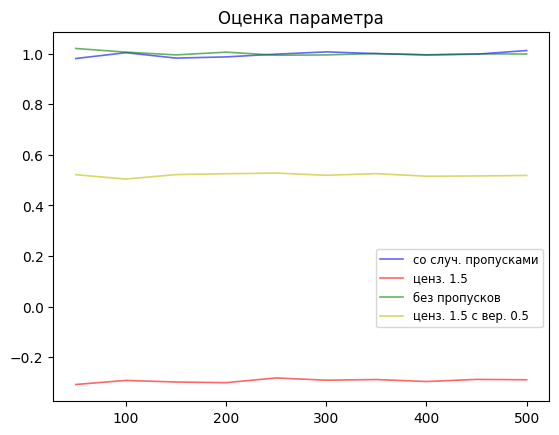
\includegraphics[width=\linewidth]{pict1.png}}
        \hfill
        \subcaptionbox*{Рисунок 2}[.49\linewidth]{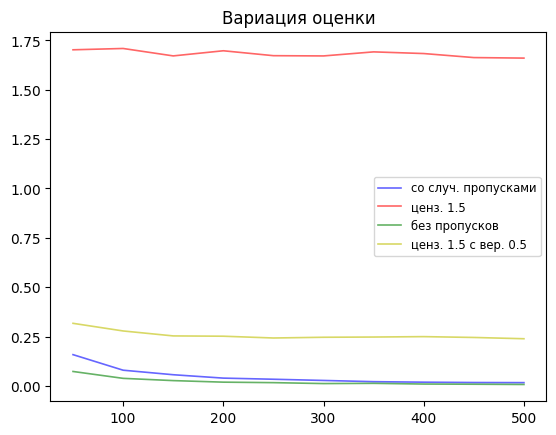
\includegraphics[width=\linewidth]{pict2.png}}
    \end{figure}

    \section{Метод максимального правдоподобия}

    Теперь попробуем применить метод максимального правдоподобия и посмотрим, насколько он усложняется в случае пропусков, 
    зависящих от данных.  
    
    Пусть дана выборка размера $n$ значений с пропусками случайной величины с плотностью вероятности $p_\xi(x,\theta)$, где  
    $\theta$ --- неизвестный параметр. И пусть модель пропусков описывается функцией $m(x)$, $Obs$ --- шаблон пропусков данной выборки, 
    $k$ --- число наблюдаемых значений выборки. Тогда функция правдоподобия (ФП) будет выглядеть следующим образом:
    \begin{equation*}
        L(\theta) = \prod_{i=1}^{n}(p_\xi(x,\theta))^{obs_i}G(p_\xi, m)^{1-obs_i},
    \end{equation*}
    где $G(p_\xi, m) = \int_{-\infty}^{+\infty}p_\xi(x, \theta)m(x)\dd x$.
    Логарифмическая ФП (ЛФП) будет иметь вид
    \begin{align*}
        l(\theta) = ln(L(\theta)) &= \sum_{i=1}^{n}obs_i \ln(p_\xi(x_i,\theta)) + (1 - obs_i)\ln(G(p_\xi,m)) = \\
                                  &= \sum_{i=1}^{n}obs_i\ln(p_\xi(x_i,\theta)) + (n-k)\ln(G(p_\xi,m)),
    \end{align*}
    где $n$ --- величина выборки, $k$ --- количество наблюдаемых значений.

    Рассмотрим три случая пропусков
    \paragraph{1. Случайные пропуски.} Рассматриваем $m(x) \equiv c,\ 0 < c < 1$ и получаем функцию $G$ и ЛФП:
    \begin{gather*}
        G(p_\xi, m) = \int_{-\infty}^{+\infty}cp_\xi(x,\theta)\dd x = c, \\
        l(\theta) = \sum_{i=1}^{n}obs_i\ln\big(p_\xi(x_i,\theta)\big) + (n-k)\ln c.
    \end{gather*}
    При случайных пропусках $G(\cdot)$ не зависит от $\theta$ и второе слагаемое никак не влияет на поиск
    максимума функции, поэтому в этом случае получение ММП-оценки никак не отличается от случая без
    пропусков.

    \paragraph{2. Цензурирование.} Рассмотрим функцию $m(x)$ вида
    \begin{equation*}
        m(x) = \begin{cases}
            0, & x < c \\
            1, & x \ge c
        \end{cases}.
    \end{equation*}
    Тогда
    \begin{gather*}
        G(p_\xi, m) = \int_{c}^{+\infty}p_\xi(x, \theta)\dd x, \\
        l(\theta) = \sum_{i=1}^{n}obs_i\ln\big(p_\xi(x_i,\theta)\big) + (n-k)\ln\big(G(p_\xi, m)\big).
    \end{gather*}
    Теперь функция $G(\cdot)$ зависит от $\theta$, что усложняет нахождение максимума функции.

    \paragraph{3. Кусочно-постоянная функция пропусков.} Для примера рассмотрим
    \begin{equation*}
        m(x) = \begin{cases}
            0, & x < a \\
            \frac12, & a \le x < b \\
            1, & x \ge b
        \end{cases}.
    \end{equation*}
    Тогда получаем ситуацию, аналогичную случаю 2:
    \begin{gather*}
        G(p_\xi, m) = \frac12\int_{a}^{b}p_\xi(x, \theta)\dd x + \int_{b}^{+\infty}p_\xi(x, \theta)\dd x, \\
        l(\theta) = \sum_{i=1}^{n}obs_i\ln\big(p_\xi(x_i,\theta)\big) + (n-k)\ln\big(G(p_\xi, m)\big).
    \end{gather*}
    Теперь рассмотрим 2 конкретных примера:

    \vspace{0.2cm}
    1. Возьмем экспоненциальное распределение
    \begin{equation*}
        p(x, \theta) = \left\{\
            \begin{array}{ll}
                \theta e^{-\theta x}, & x \geq 0 \\
                0, & x < 0
            \end{array}\right., \quad \theta > 0
    \end{equation*} 
    и модель пропусков
    \begin{equation*}
        m(x) = \left\{\
            \begin{array}{ll}
                0, & x < 0 \\
                \frac12, & 0 \leq x \leq 3 \\
                0, & x > 3
            \end{array}\right. .
    \end{equation*}
    Тогда
    \begin{equation*}
        G(p, m) = \int_{0}^{3}\frac{\theta}{2}e^{-\theta x}\dd x = \frac12 (1 - e^{-3\theta})
    \end{equation*}
    и
    \begin{equation*}
        L(\theta) = \theta^k e^{-\theta\sum_{obs_i = 1}}\frac{1}{2^{n-k}}(1 - e^{-3\theta})^{n - k}.
    \end{equation*}

    Прологарифмируем функцию правдоподобия и вычислим производную для поиска точки максимума
    \begin{equation*}
        l(\theta) = \ln L(\theta) = k\ln\theta - \theta\sum_{obs_i = 1}x_i + (n - k)\ln\left(\frac12(1 - e^{-3\theta})\right),
    \end{equation*}
    \begin{equation*}
        l'(\theta) = \frac{k}{\theta} - \sum_{obs_i = 1}x_i + 3(n - k)\left(\frac{1}{1 - e^{-3\theta}} - 1\right).
    \end{equation*}

    Перенесем все слагаемые с $\theta$ влево и получим уравнение для нахождения МП-оценки параметра
    \begin{equation*}
        \frac{k}{\theta} + \frac{1}{1 - e^{-3\theta}} = \sum_{obs_i = 1}x_i - 3(n - k).
    \end{equation*}

    Уравнение уже слишком сложное для аналитического решения, параметр можно оценить только численными методами, приближенно. 

    \vspace{0.2cm}
    2. Возьмем нормальное распределение
    \begin{equation*}
        p(x, \theta) = \frac{1}{\sqrt{2\pi}\sigma}e^{-\frac{(x-a)^2}{2\sigma^2}}
    \end{equation*}
    и ту же модель пропусков, что и в прошлом примере. Тогда
    \begin{equation*}
        G(p, m) = \frac{1}{2\sqrt{2\pi}\sigma}\int_{0}^{3} e^{-\frac{(x-a)^2}{2\sigma^2}} \dd x,
    \end{equation*}
    \begin{align*}
        L(a, \sigma) &= \prod_{i=1}^{n} \left(\frac{1}{\sqrt{2\pi}\sigma}e^{-\frac{(x-a)^2}{2\sigma^2}}\right)^{obs_i} 
        \left(\frac{1}{2\sqrt{2\pi}\sigma}\int_{0}^{3} e^{-\frac{(x-a)^2}{2\sigma^2}} \dd x\right)^{1 - obs_i} = \\ 
                    &= \left(\frac13\right)^{n-k}\left(\frac{1}{\sqrt{2\pi}\sigma}\right)^n e^{-\sum_{obs_i}\frac{(x_i - a)^2}{2\sigma^2}}
    \end{align*}
    Функция правдоподобия уже стала настолько сложной, что даже взятие производной затруднительно. Поэтому здесь оценка параметров является препятствием даже для численных методов.
    
    Посмотрим, какими методами можно найти значения параметров проще.


    \section{Метод моментов}

    Первым из методов, которые мы рассмотрим, будет метод моментов. Он основан на приравнивании теоретических характеристик распределения к выборочным. В случае пропусков, зависящих от данных, удобнее всего использовать следующие два равенства
    \begin{gather*}
        P\{obs_i = 1\} = \int_{-\infty}^{+\infty}p_\xi(x,\theta)(1 - m(x))\dd x = \frac{k}{n}, \\
        E\{x_i\} = \frac{\int_{-\infty}^{+\infty}xp_\xi(x,\theta)(1-m(x))\dd x}{\int_{-\infty}^{+\infty}p_\xi(x,\theta)(1-m(x))\dd x} = \frac{\sum_{obs_i = 1}x_i}{k},
    \end{gather*}
    где $k$ --- количество наблюдаемых значений в выборке.

    Сначала посмотрим, как изменится вид уравнений в различных случаях с пропусками.

    \paragraph{1. Случайные пропуски.} В этом случае $m(x) \equiv c,\ 0 < c < 1$ и уравнения 
    примут следующий вид
    \begin{gather*}
        \frac{k}{n} = \int_{-\infty}^{+\infty}p_\xi(x,\theta)(1-m(x))\dd x = 
            (1-c)\int_{-\infty}^{+\infty}p_\xi(x,\theta)\dd x = 1-c \\
        \frac{\sum_{obs_i = 1}x_i}{n} = 
            \frac{\int_{-\infty}^{+\infty}xp_\xi(x,\theta)(1-m(x))\dd x}%
                {\int_{-\infty}^{+\infty}p_\xi(x,\theta)(1-m(x))\dd x} = E\{\xi\}
    \end{gather*}
    Из первого уравнения пропала $\theta$, поэтому его нельзя использовать. Вместо него можно
    составить уравнение для момента порядка 2 или выше. Второе же уравнение в итоге ничем не отличается от
    соответствующего уравнения в случае без пропусков.

    \paragraph{2. Цензурирование.} Рассматриваем функцию вероятности пропуска
    \begin{equation*}
        m(x) = \begin{cases}
            0, & x < c \\
            1, & x \ge c
        \end{cases}.
    \end{equation*}
    В таком случае уравнения примут вид
    \begin{gather*}
        \int_{-\infty}^{c}p_\xi(x,\theta)\dd x = \frac{k}{n}, \\
        \frac{\int_{-\infty}^{c}xp_\xi(x,\theta)\dd x}{\int_{-\infty}^{c}p_\xi(x,\theta)\dd x} = \frac{\sum_{obs_i = 1}x_i}{n}
    \end{gather*}

    \paragraph{3. Кусочно-постоянная функция пропусков.} К примеру, возьмем функцию
    \begin{equation*}
        m(x) = \begin{cases}
            0, & x < a \\
            \frac12, & a \le x < b \\
            1, & x \ge b
        \end{cases}.
    \end{equation*}
    Подставив в уравнения баланса, получим
    \begin{gather*}
        \int_{-\infty}^{a}p_\xi(x,\theta)\dd x + \frac12\int_{a}^{b}p_\xi(x,\theta)\dd x = \frac{k}{n} \\
        \frac{\int_{-\infty}^{a}xp_\xi(x,\theta)\dd x + \frac12\int_{a}^{b}xp_\xi(x,\theta)\dd x}%
            {\int_{-\infty}^{c}p_\xi(x,\theta)\dd x + \frac12\int_{a}^{b}p_\xi(x,\theta)\dd x} = \frac{\sum_{obs_i = 1}x_i}{n}
    \end{gather*}
    Для решения сначала применим метод к распределению с одним параметром, например к экспоненциальному
    \begin{equation*}
        p(x,\theta) = \begin{cases}
                \theta e^{-\theta x}, &  x \ge 0 \\
                0,                    &  x < 0 
            \end{cases}, \quad \theta > 0.
    \end{equation*}
    В случаях 2 и 3 уравнения усложняются, в особенности тем, что во втором уравнении слева имеем частное
    двух интегралов, зависящих от $\theta$. 

    Теперь проверим метод моментов на практике. Возьмем параметр $\theta = 1$ и функцию модели пропусков
    \begin{equation*}
        m(x) = \begin{cases}
                1,       & x < 1 \\
                \frac12, & 1 \le x \le 2 \\
                0,       & x > 2
            \end{cases}
    \end{equation*}
    и проведем компьютерный эксперимент, аналогичный тому, который проводился для метода <<игнорирования пропусков>>. 
    Замечу, что здесь достаточно только одного из двух уравнений метода моментов. В таком случае можно решать его методом дихотомии, предполагая, что функция зависимости интеграла $\int_{-\infty}^{+\infty}p_\xi(x,\theta)m(x)\dd x$ от параметра $\theta$ монотонна.

    На рисунках 3 и 4 показаны оценки и их вариация для разных объемов выборки.
    \begin{figure}[H]
        \subcaptionbox*{Рисунок 3}[.49\linewidth]{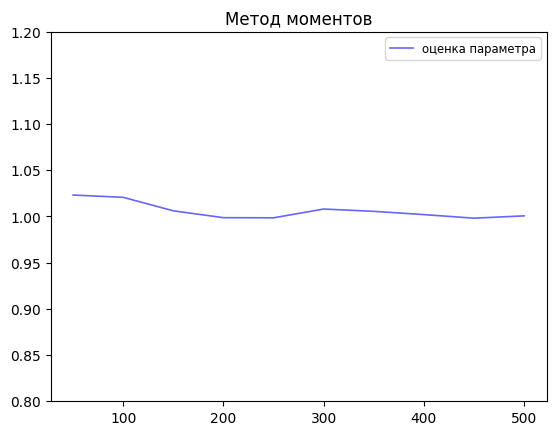
\includegraphics[width=\linewidth]{pict3.png}}
        \hfill
        \subcaptionbox*{Рисунок 4}[.49\linewidth]{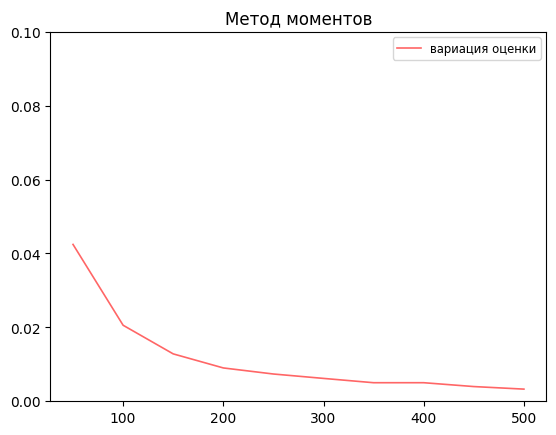
\includegraphics[width=\linewidth]{pict4.png}}
    \end{figure}
    Как видим, метод достаточно точен и даже при небольшом объеме выборки средняя вариация не превысила значения 0.05.

    Теперь попробуем таким же образом применить этот метод к нормальному распределению c параметрами $a = 0.7$ и $\sigma = 0.8$. 
    Так как параметра два, придется решать систему из двух уравнений, приведенных в начале главы. Это гораздо сложнее, чем в случае с одним параметром, поэтому для нахождения решения использовались инструменты языка Python (в котором реализован метод сопряженных направлений).

    На рисунках 5 и 6 показаны оценка и вариация соответственно для параметров распределения. Видим, что для нормального распределения метод тоже работает.
    \begin{figure}[H]
        \subcaptionbox*{Рисунок 5}[.49\linewidth]{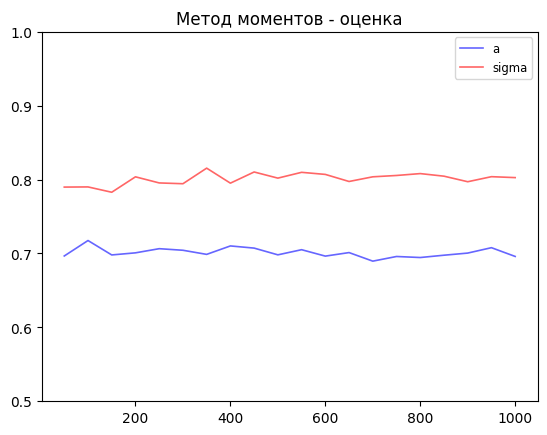
\includegraphics[width=\linewidth]{pict5.png}}
        \hfill
        \subcaptionbox*{Рисунок 6}[.49\linewidth]{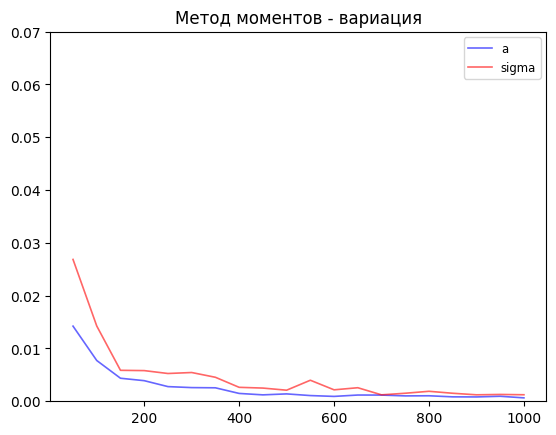
\includegraphics[width=\linewidth]{pict6.png}}
    \end{figure}

    \section{Заключение}

    Таким образом, в курсовой работе получены следующие основные результаты:
    \begin{enumerate}
        \item Произведено сравнение поведения оценок параметров распределения вероятности, полученных методом игнорирования пропусков, для различных видов пропусков во временном ряду. Показана несостоятельность метода в случае неслучайных пропусков. 
        \item На примере метода максимального правдоподобия исследовано влияние, оказываемое на стандартные методы получения оценок параметров смешением плотности распределения вероятности с функцией модели пропусков, зависящих от данных.
        \item Исследованы методы, позволяющие получить верные оценки параметров распределения для случая неслучайных пропусков.
    \end{enumerate}

    % \begin{thebibliography}{9}
    \bibitem{1}
    Андерсон, Т. Статистический анализ временных рядов / Т. Андерсон --- М.: Мир, 1976. --- 755 с.

    \bibitem{2}
    Дженкинс, Г., Ваттс, Д. Спектральный анализ и его приложения: в 2 т. / Г. Дженкинс, Д. Ваттс М.: МирГод, --- 1971. --- Т. 1. --- 317 с.

    \bibitem{3}
    Бокс Дж., Дженкинс Г. Анализ временных рядов, прогноз и управление / Под ред. Писаренко В. Ф. --- М.: Мир, 1974, кн. 1. --- 406 с. 

    \bibitem{4}
    Эконометрия / В. И. Суслов [и др.] --- Новосибирский государственный университет, 2005. --- 744 с.

    \bibitem{5}
    Криптология: учебник / Ю. С. Харин [и др.] --- Минск: БГУ, 2013. – 511 с. --- (Классическое университетское издание).

    \bibitem{6}
    Харин, Ю.С. Оптимальность и робастность в статистическом прогнозировании / Ю. С. Харин --- Минск: БГУ, 2008. --- 263 с: ил.

    \bibitem{7}
    Харин, Ю. С. Теория вероятностей, математическая и прикладная статистика: учебник / Ю. С. Харин, Н. М. Зуев, Е. Е. Жук. --- Минск: БГУ, 2011. --- 463 с. --- (Классическое университетское издание).

    \bibitem{8}
    Zhidong, B. Statistical analysis for rounded data / Z, Shurong, Z. Baoxue, Hu Guorong // Journal of Statistical Planning and Inference. --- 2009 Vol. 139, No. 8. --- P. 2526-2542.

    \bibitem{9}
    Park, J.W. Censored time series analysis with autoregressive moving average models. / J.W. Park, M.G. Genton, S.K. Ghosh // The Canadian journal of statistics. --- 2007.  --- Vol. 35, No. 1. --- P. 151-168.
\end{thebibliography}

    % \section{Приложение А. Листинг программы}
        \begin{minted}[autogobble]{python}
            import numpy as np
            from scipy.stats import norm
            import matplotlib.pyplot as plt
            import random as random

            def omit_rand(data, prob):
                temp = np.empty(data.size)
                for i in range(data.size):
                    temp[i] = data[i]
                    rand = random.random()
                    if rand < prob:
                        temp[i] = np.nan
                return temp

            def omit_cens(data, border, prob):
                temp = np.empty(data.size)
                for i in range(data.size):
                    temp[i] = data[i]
                    rand = random.random()
                    if data[i] > border and rand < prob:
                        temp[i] = np.nan
                return temp

            def eval_params_avg(data):
                temp = np.empty(data.size - np.count_nonzero(np.isnan(data)))
                i = 0
                for num in data:
                    if not np.isnan(num):
                        temp[i] = num
                        i += 1

                sum = 0
                for num in temp:
                    sum += num
                avg = sum / temp.size
                return avg

            def calc_loc_err(msize, mloc, mscale, mborder, mprob):
                err_sum = 0
                am = 500
                for i in range(am):
                    data = norm.rvs(size=msize, loc=mloc, scale=mscale)
                    data = omit_cens(data, mborder, mprob)
                    err_sum += (eval_params_avg(data) - mloc)**2
                err_sum /= am
                return err_sum


            def calc_loc_err_rnd(msize, mloc, mscale, mprob):
                err_sum = 0
                am = 500
                for i in range(am):
                    data = norm.rvs(size=msize, loc=mloc, scale=mscale)
                    data = omit_rand(data, mprob)
                    err_sum += (eval_params_avg(data) - mloc)**2
                err_sum /= am
                return err_sum

            def calc_loc_err_no(msize, mloc, mscale):
                err_sum = 0
                am = 500
                for i in range(am):
                    data = norm.rvs(size=msize, loc=mloc, scale=mscale)
                    err_sum += (eval_params_avg(data) - mloc)**2
                err_sum /= am
                return err_sum

            def calc_loc(msize, mloc, mscale, mborder, mprob):
                sum = 0
                am = 500
                for i in range(am):
                    data = norm.rvs(size=msize, loc=mloc, scale=mscale)
                    data = omit_cens(data, mborder, mprob)
                    sum += eval_params_avg(data)
                sum /= am
                return sum

            def calc_loc_rnd(msize, mloc, mscale, mprob):
                sum = 0
                am = 500
                for i in range(am):
                    data = norm.rvs(size=msize, loc=mloc, scale=mscale)
                    data = omit_rand(data, mprob)
                    sum += eval_params_avg(data)
                sum /= am
                return sum


            fig, ax = plt.subplots(1, 1)

            ax.plot(x4, y4, 'b-', lw=1.2, alpha=0.6, label='со случ. пропусками')
            ax.plot(x, y, 'r-', lw=1.2, alpha=0.6, label='ценз. 1.5')
            ax.plot(x2, y2, 'g-', lw=1.2, alpha=0.6, label='без пропусков')
            ax.plot(x7, y7, 'y-', lw=1.2, alpha=0.6, label='ценз. 1.5 с вер. 0.5')

            plt.title('Вариация оценки')
            plt.legend(fontsize='small')
            plt.show()

            fig, ax = plt.subplots(1, 1)
            ax.plot(x6, y6, 'b-', lw=1.2, alpha=0.6, label='со случ. пропусками')
            ax.plot(x1, y1, 'r-', lw=1.2, alpha=0.6, label='ценз. 1.5')
            ax.plot(x5, y5, 'g-', lw=1.2, alpha=0.6, label='без пропусков')
            ax.plot(x3, y3, 'y-', lw=1.2, alpha=0.6, label='ценз. 1.5 с вер. 0.5')

            plt.title('Оценка параметра')
            plt.legend(fontsize='small', loc=(0.65,0.2))
            plt.show()

        \end{minted}

\end{document}